%
Concettualmente, un valore di un tipo interfaccia, o \textit{valore di interfaccia}, ha due componenti, un tipo concreto e un valore di quel tipo.
Queste sono dette \textit{tipi dinamici} e \textit{valori dinamici} di interfaccia.

Per un linguaggio staticamente tipizzato come Go, i tipi sono un concetto a compile-time, così un tipo non è un valore.
In un modello concettuale, un insieme di valori detto \textit{descrittori di tipo} forniscono informazioni su ogni tipo, come il suo nome e i suoi metodi.
In un valore di interfaccia, il componente del tipo è rappresentato dal descrittore di tipo appropriato.

Nelle seguenti istruzioni, la variabile \verb|w| assume tre valori differenti.
\begin{lstlisting}[frame=single, label={lst:lstlisting6-5.1}]
var w io.Writer
w = os.Stdout
w = new(bytes.Buffer)
w = nil
\end{lstlisting}
Vediamo nel dettaglio cosa accade dopo l'esecuzione di ogni istruzione.
Il primo dichiara \verb|w|:
\begin{lstlisting}[frame=single, label={lst:lstlisting6-5.2}]
var w io.Writer
\end{lstlisting}
In Go, le variabili sono sempre inizializzate ad un valore ben definito, e le interfacce non fanno eccezione.
Il valore zero di un interfaccia ha sia i tipi che i valori dei suoi componenti impostati a \verb|nil|.
\begin{center}
    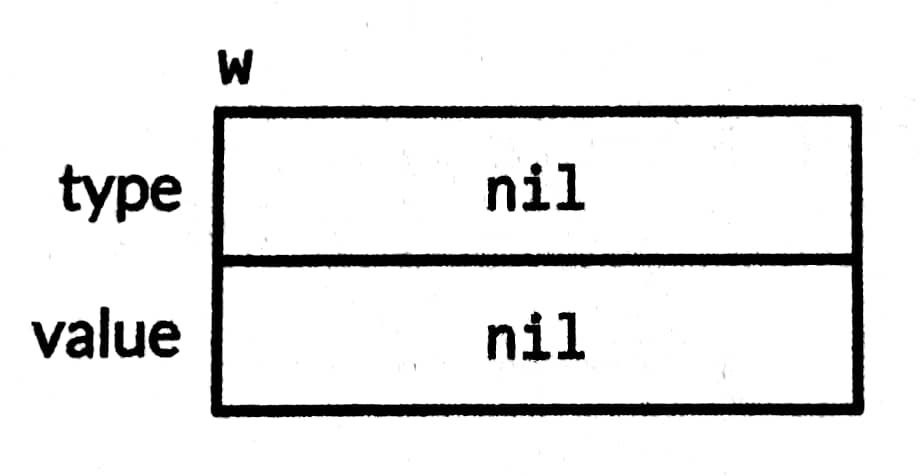
\includegraphics[width=0.4\linewidth]{figures/figura6.1}
\end{center}

Un valore interfaccia è descritto come nil o non-nil a seconda del suo tipo dinamico.

La seconda istruzione assegna un valore di tipo \verb|*os.File| a \verb|w|:
\begin{lstlisting}[frame=single, label={lst:lstlisting6-5.3}]
w = os.Stdout
\end{lstlisting}
Questo assegnamento coinvolge una conversione implicita da un tipo concreto al tipo di interfaccia, ed è equivalente alla conversione esplicita \verb|io.Writer(os.Stdout)|.
Una conversione di questo tipo cattura il tipo e il valore dei suoi operandi.
Il tipo dinamico del valore di interfaccia è impostato al descrittore del tipo per un tipo puntatore \verb|*os.File|, e il suo valore dinamico detiene una copia di \verb|os.Stdout|, che è un puntatore ad una variabile \verb|os.File| rappresentante lo standard output di un processo.
\begin{center}
    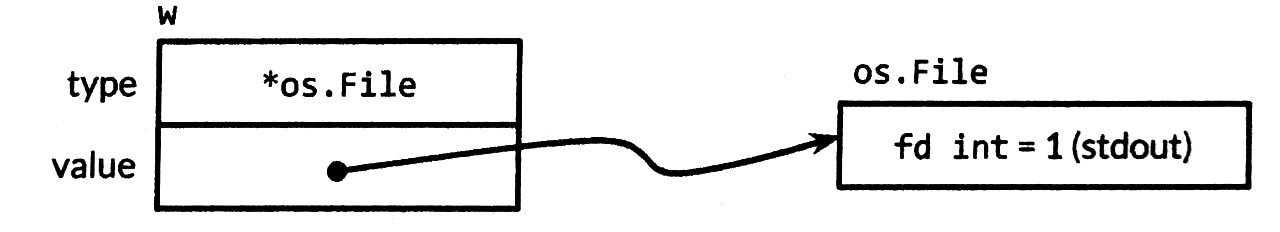
\includegraphics[width=0.5\linewidth]{figures/figura6.2}
\end{center}

In generale, non è possibile conoscere a compile-time quale tipo dinamico del valore di interfaccia sarà, così una chiamata tramite un interfaccia deve usare un \textit{invio dinamico}.
Invece di una chiamata diretta, il compilatore deve generare codice per ottenere l'indirizzo del metodo \verb|Write| dal tipo del descrittore, quindi produrre una chiamata indiretta a quel indirizzo.
L'argomento ricevitore per la chiamata è una copia del valore dinamico dell'interfaccia, \verb|os.Stdout|.
L'effetto è come se si fosse prodotta una chiamata direttamente.

La terza istruzione assegna un valore di tipo \verb|*bytes.Buffer| al valore di interfaccia:
\begin{lstlisting}[frame=single, label={lst:lstlisting6-5.4}]
w = new(bytes.Buffer)
\end{lstlisting}
Il tipo dinamico è ora \verb|*bytes.Buffer| e il valore dinamico è un puntatore al nuovo buffer allocato.
\begin{center}
    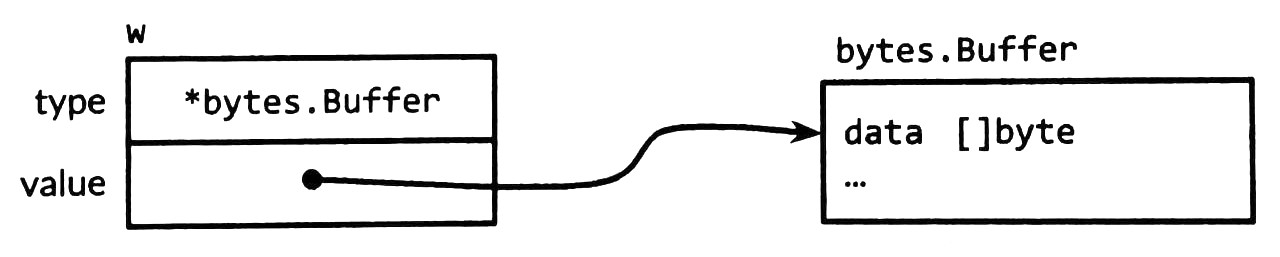
\includegraphics[width=0.5\linewidth]{figures/figura6.3}
\end{center}

Infine, la quarta istruzione assegna \verb|nil| al valore di interfaccia:
\begin{lstlisting}[frame=single, label={lst:lstlisting6-5.5}]
w = nil
\end{lstlisting}
Questo fa il reset di entrambi i suoi componenti a \verb|nil|, ripristinando \verb|w| allo stato della sua dichiarazione.

I valori di interfaccia possono essere confrontati usando \verb|==| e \verb|!=|, quindi utilizzabili anche come chiavi per le map o come gli operandi di un'istruzione switch.
Bisogna comunque fare attenzione, perché se le interfacce hanno stessi tipi dinamici, ma non confrontabili tra loro, allora il confronto fallisce con il lancio di un panic.
\begin{lstlisting}[frame=single, label={lst:lstlisting6-5.6}]
var x interface{} = []int{1, 2, 3}
fmt.Println(x == x) // panic: i tipi []int non sono
                    // confrontabili
\end{lstlisting}
Per questi motivi in generale si possono confrontare i valori di un interfaccia se si è certi che questo contenga valori dinamici di tipi confrontabili.